\section{Unterschiedliche Charakter}
Spiele verwenden die unterschiedlichsten Charaktere, nicht nur in Bezug auf das Aussehen, sondern auch hinsichtlich der Komplexität der Körperteile und der Anzahl der Knochen. Um den Charaktercontroller vielseitig einsetzbar zu gestalten, werden in diesem Kapitel die Walker-Demo-Komponenten angepasst, um den Einrichtungsprozess zu vereinfachen und unterschiedliche Charakterkörperstrukturen zu ermöglichen. Zunächst wird analysiert, wie das Agentenskript angepasst werden muss, um Charaktere mit unterschiedlichen Körperstrukturen zu steuern und zu trainieren. Anschließend wird der Einrichtungsprozess am Beispiel eines Mixamo-3D-Charaktermodells dargestellt. Zum Schluss wird der Mixamo-Charakter trainiert und das Ergebnis ausgewertet. Die Wahl des Mixamo-Modells als Beispiel soll zeigen, wie die Einrichtung mit den Vereinfachungen funktioniert und wie das Training bei der Verwendung von komplexere Charaktermodelle beeinflusst wird.

\subsection{Anforderungen}	
Der Agent der Walker Demo setzt für jedes Körperteil eine separate Referenz, die über den Inspector in Unity konfiguriert werden muss. Um die damit verbundene Einschränkung einer festgelegten Konfiguration von Körperteilen zu beheben, soll eine flexible Liste von Körperteilen konfiguriert werden. Bei der Zustandserfassung der Körperteile soll anschließend der Zustand aller Körperteile in der Liste erfasst werden. Die Aktion soll gleichermaßen Zielwinkel und Gelenkstärke für alle Körperteile der Liste beinhalten. Um unnötige Komplexität bei der Beobachtung und Aktion zu vermeiden, sollen die Zielwinkel nur für bewegbare Gelenkachsen bestimmt werden. Die Gelenkstärke soll für komplett versteifte Gelenke ebenfalls ausgelassen werden. Um die Konfiguration weiter zu erleichtern, sollen die Körperteile zudem automatisch dem Walker-Agenten hinzugefügt werden. Schließlich soll auch das \hl{Stabilisierungsobjekt} automatisch generiert werden. Diese Änderungen zielen darauf ab, die Flexibilität und Benutzerfreundlichkeit des Walker-Demo-Agenten zu verbessern. Es soll manuelle Konfiguration auf das nötigste reduziert werden, gleichzeitig soll aber auch eine Skalierbare Lösung für unterschiedliche Charakterkörperstrukturen implementiert werden.

\subsection{Anpassungen}
Um ein Objekt als Körperteil zu definieren, wurde die Bodypart-Klasse in ein MonoBehaviour-Unity-Skript umgewandelt. Als MonoBehaviour kann das Skript im Unity Editor jedem beliebigen Objekt hinzugefügt werden. Zusätzlich wurden die Funktionen zur Steuerung der Körperteile von der Gelenk-Motor-Steuerung in das Körperteil-Skript verlagert. Dadurch ist es möglich, die Körperteile direkt über das Körperteil-Skript zu steuern, ohne den Umweg über die Gelenk-Motor-Steuerung. Die Körperteilkomponente initialisiert sich beim Programmstart und ist anschließend sowohl für die Steuerung als auch für die Aktualisierung der Zustandsparameter des Körperteils zuständig. Jedes Körperteil benötigt eine Festkörperkomponente. Zusätzlich wird überprüft, ob das Objekt über eine Gelenkkomponente verfügt. Existiert eine solche Komponente, wird diese eingerichtet und die Freiheitsgrade bestimmt. Diese Freiheitsgrade geben an, welche Felder für das Körperteil in der Beobachtung und Aktion hinzugefügt werden müssen.

Der Walker-Agent sucht beim Programmstart alle Körperteile und speichert sie in einer Liste ab. Beim Erstellen der Beobachtung und beim Umwandeln der Aktion in eine Bewegung wird über die Körperteilliste iteriert, und für jedes Körperteil wird die entsprechende Beobachtung erstellt oder die Aktion ausgeführt.
Das \hl{Stabilisierungsobjekt} wird auch automatisch beim initialisieren des Agenten erstellt.

\begin{figure}[H]
  \centering  
  \begin{tikzpicture}[node distance=3cm]
  
    \node(oc) [rounded] {Stabilisierungsobjekt};  
    \node(agent) [rounded, below of=oc] {Agent};
    \node(target) [rounded, left of=agent, xshift=-2cm] {Ziel};
    \node(jdc) [rounded, below of=agent] {Motor Gelenk Steuerung};
    \node(bp) [rounded, right of=jdc, xshift=3cm] {Körperteil};
    \node(gc) [rounded, right of=agent, xshift=4cm] {Bodenkontakt};
    
    \draw [uni] (agent) -- (oc) node[midway, right] {aktualisiert Ausrichtung};
    \draw [uni] ([shift={(0.5,-0.5)}] agent.center) -- ([shift={(0.5,0.5)}] jdc.center) node[midway, right] {init Körperteile};
    \draw [uni] ([shift={(-0.5,0.5)}] jdc.center) -- ([shift={(-0.5,-0.5)}] agent.center) node[midway, left, align=center] {Körperteil-\\liste};
    \draw [uni] (jdc) -- (bp) node[midway, above] {init};
    \draw[uni] ([shift={(0, 0.3)}] gc.west) -- ([shift={(0, 0.3)}] agent.east) node[midway, above] {frühes stoppen};
    \draw [uni] ([shift={(0, -0.3)}] agent.east) -| ([shift={(-1,0.5)}] bp.center) node[midway, left, yshift=-0.2cm] {steuert};
    \draw[uni] ([shift={(1,0)}] bp.north) -- (gc) node[midway, right] {hat};
    \draw [uni] (target) to[loop below] () node [yshift=-1.5cm, align=center] {setzt neue\\Position};
        
  \end{tikzpicture}
  \caption{Alte Architektur}
  \label{fig:architektur_alt}
\end{figure}

\begin{figure}[H]
  \centering  
  \begin{tikzpicture}[node distance=3cm]
  
    \node(oc) [rounded] {Stabilisierungsobjekt};  
    \node(agent) [rounded, below of=oc] {Agent};
    \node(target) [rounded, left of=agent, xshift=-2cm] {Ziel};
    \node(bp) [rounded, right of=agent, xshift=3cm] {Körperteil};
    
    \draw [uni] (oc) to[loop above] () node[yshift=1.5cm] {aktualisiert Ausrichtung};
    \draw [uni] (agent) -- (oc) node[midway, right] {erstellt};
    \draw [uni] ([shift={(0,0.3)}]  agent.east) -- ([shift={(0,0.3)}] bp.west) node[midway, above] {steuert};
    \draw [dashed,uni] ([shift={(0,-0.3)}] bp.west) -- ([shift={(0,-0.3)}] agent.east) node[midway, below, align=center] {Event\{bodenkontakt\\Zielberührung\}};
    \draw[uni] (agent) to[loop below] () node[yshift=-1.5cm] {frühes stoppen};
    \draw [dashed, uni] (agent) -- (target) node[midway, above, align=center] {Event\{setzt neue\\Position\}};
        
  \end{tikzpicture}
  \caption{Neue Architektur}
  \label{fig:architektur_neu}
\end{figure}

\subsection{Einrichtung}
Der ausgewählte Charakter ist der Y Bot Charakter welcher in Abbildung \ref{fig:charakter_mixamo} zu sehen ist. Der Y Bot besteht ausgenommen der Finger aus 22 Knochen. Um das Training zu beschleunigen werden für alle Versuche die Finger mit dem Handknochen als ein Körperteil zusammengefasst.

\begin{figure}[H]
  \centering  
  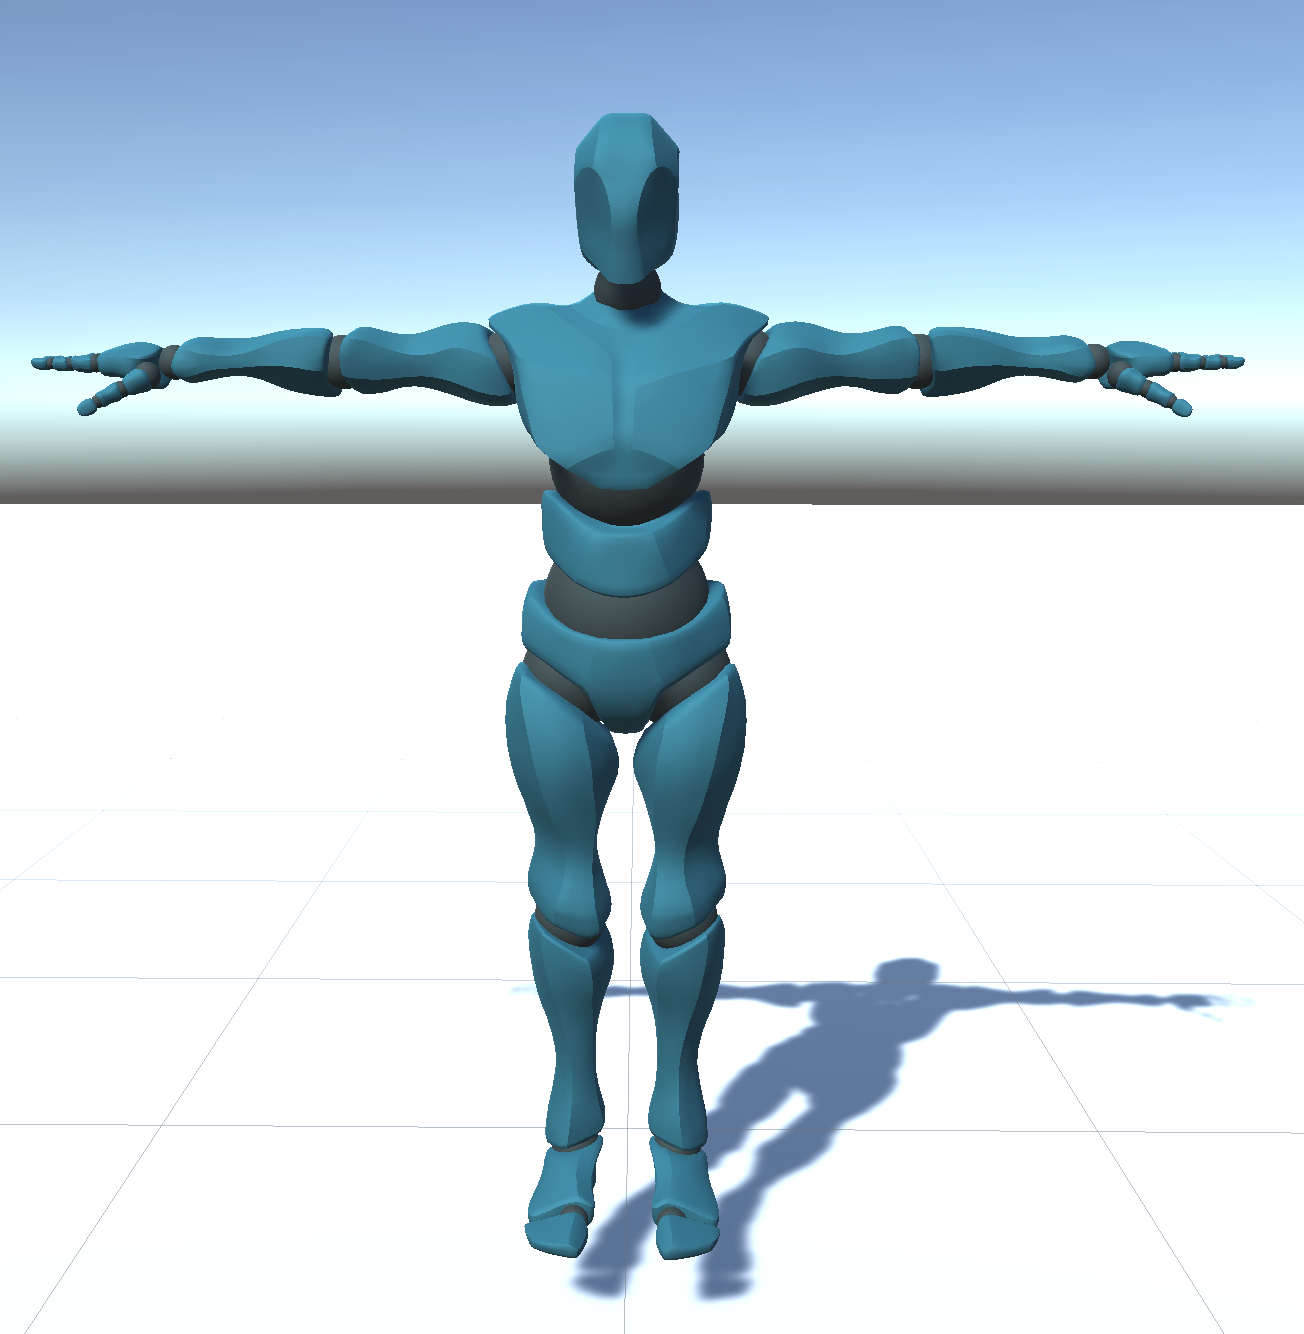
\includegraphics[scale=0.5]{img/charakter_mixamo}
  \caption{Mixamo Charakter Y Bot}
  \label{fig:charakter_mixamo}
\end{figure}

Jedes Körperteil benötigt für das Steuern und Trainieren mit dem Walker Agenten Skript eine Kollisionskomponente, eine Festkörperkomponente und eine Körperteilkomponente. Zusätzlich müssen Gelenkkomponenten hinzugefügt werden, um die Körperteile miteinander zu verbinden. Dabei wird die Gelenkkomponente jeweils auf das untergeordnete Körperteil angewendet, während das übergeordnete Körperteil als verbundener Körper referenziert wird. Die Kollisionskomponente soll das Körperteil in vereinfachter Form und Größe darstellen, um die Berechnungen zu optimieren. Bei den Festkörpern müssen das Gewicht und der Schwerpunkt festgelegt werden, um eine realistische physikalische Simulation zu gewährleisten. In der Gelenkkomponente können Bewegungen durch das Festlegen von Winkellimits gesperrt oder limitiert werden. Für die Rotationsberechnung wird der Slerp-Modus verwendet, \hl{da dieser eine gleichmäßige Interpolation der Rotation ermöglicht}. DieKörperteilkomponente übernimmt die Konfigurationsparameter der Gelenk Motor Steuerung (siehe Abbildung \ref{fig:komponente_bodypart}. Parameter wie Stärke und maximale Rotationsgeschwindigkeit können angepasst werden, wobei die Standardwerte aus der Walker Demo in den meisten Fällen ausreichend sind. Bei Bedarf kann auch das Feld \grqq{}Trigger Touching Ground\grqq{} aktiviert werden, um ein Event auszulösen, sobald das Körperteil den Boden berührt.

\begin{figure}[H]
  \centering  
  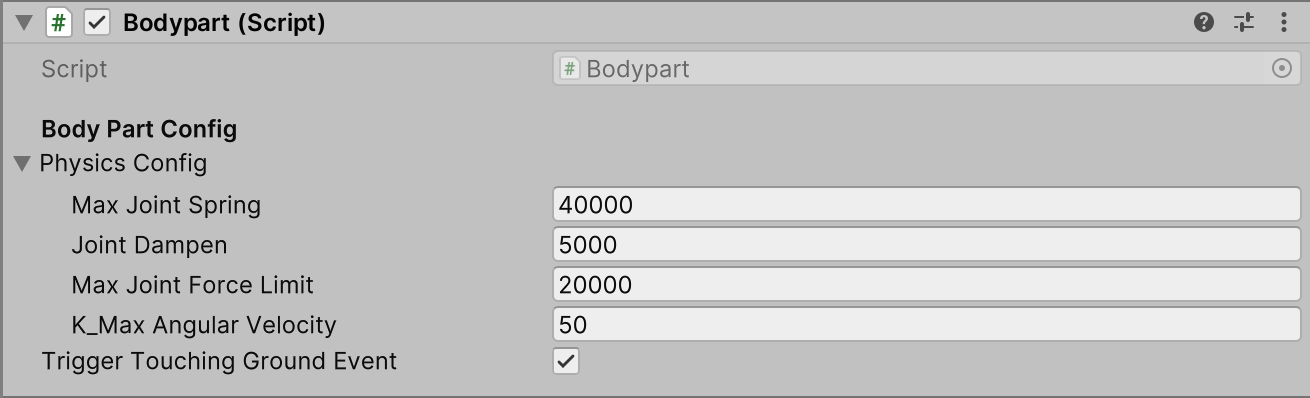
\includegraphics[scale=0.5]{img/komponente_bodypart}
  \caption{Körperteilkomponente}
  \label{fig:komponente_bodypart}
\end{figure}


Ist der Körper fertig konfiguriert wird zuletzt das Walker Agent Skript, die Behaviour Parameter und der Decision Requester hinzugefügt. 

\begin{figure}[H]
  \centering  
  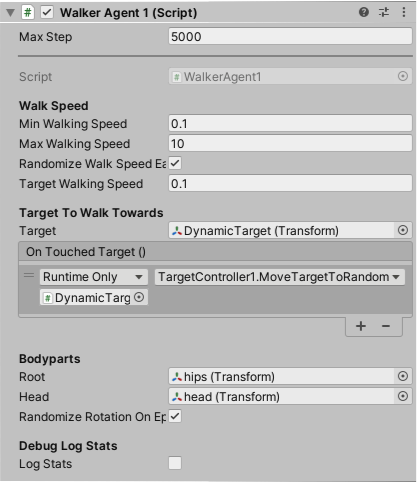
\includegraphics[scale=0.5]{img/komponente_agent_walker1}
  \caption{Walker Agentkomponente}
  \label{fig:komponente_agent_walker1}
\end{figure}

Die Gewichte der Körperteile wurden von der Walker Demo übernommen. Gleichermaßen wurden die Winkellimits für die Gelenke übernommen. Die zusätzlichen Körperteile wurden vereinfacht. Der Oberkörper besteht im Mixamo Modell aus den Schulterknochen sowie dem obersten Wirbel der Wirbelsäule. Die Wirbelsäule besteht im Mixamo Modell aus 2 Wirbeln anstatt dem einen Wirbel des Läufers aus der Demo. Zuletzt sind die Füße noch in Fuß und Vorderfuß aufgeteilt. Bei diesen Änderungen der Körperstruktur wurden die Gewichte und Winkellimits des vereinfachten Körpers auf die komplexeren Körperstrukturen aufgeteilt.

\begin{table}[H]
  \centering
  {\rowcolors{1}{gray!10}{white}
  \begin{tabular}{ |p{3cm}|p{3cm}|p{2cm}|p{4cm}|p{2cm}| }
  \hline
  \textbf{Körpertei}l& \textbf{Verbundenes Körperteil} & \textbf{Gewicht} & \textbf{Winkellimits} & \textbf{Form} \\
  \hline
  Hüfte & - & 15kg & - & Kapsel \\
  \hline
  Wirbel 1 & Hüfte & 6kg & x(-20,20) y(-20,20) z(-15,15) & Kugel \\
  \hline
  Wirbel 2 & Wirbel 1 & 4kg & - & Kugel \\
  \hline
  Wirbel 3 & Wirbel 2 & 3kg & x(-20,20) y(-20,20) z(-15,15) & Kugel \\
  \hline
  Schulter LR & Wirbel 3 & je 2kg& - & Kugel \\
  \hline
  Nacken & Wirbel 3 & 1kg & - & Kugel \\
  \hline
  Kopf & Nacken & 6kg & x(-30,10) y(-20,20) & Kapsel \\
  \hline
  Oberarm LR & Oberkörper & je 4kg & x(-60,120) y(-100,100) & Kapsel \\
  \hline
  Unterarm LR & Oberarm & je 3kg & x(0,160) & Kapsel \\
  \hline
  Hand LR & Unterarm & je 2kg & - & Quader \\
  \hline
  Oberschenkel LR & Hüfte & je 14kg& x(-90,60) y(-40,40) & Kapsel \\
  \hline
  Unterschenkel LR & Oberschenkel & je 7kg &  x(0,120) & Kapsel \\
  \hline
  Fuß LR & Unterschenkel & je 4kg & x(-20,20) y(-20,20) z(-20,20) & Quader \\
  \hline
  Vorderfuß LR & Fuß & je 1kg & - & Quader \\
  \hline
  \end{tabular}}
  \caption{Mixamo Charakter Körperteile}
  \label{table:mixamo_körperteile}
\end{table}

\subsection{Auswertung}
Das Training dauert etwa doppelt so lange um ein etwas schlechteres Resultat zu erreichen. Der Agent lernt mit dem Mixamo Modell lange in der Umgebung zu bestehen und erreicht dabei auch ein gutes Maß an Belohnung pro Schritt (siehe Abbildung \ref{fig:training_mixamo_charakter}). In der Abbildung \ref{fig:mixamo_versuch10_gangbild} wird das erlernte Gangbild gezeigt. Der Läufer lernt in diesem Fall nicht das Laufen sondern galoppiert zum Ziel.

\begin{figure}[H]
  \centering  
    \begin{subfigure}{.49\textwidth}
      \centering  
      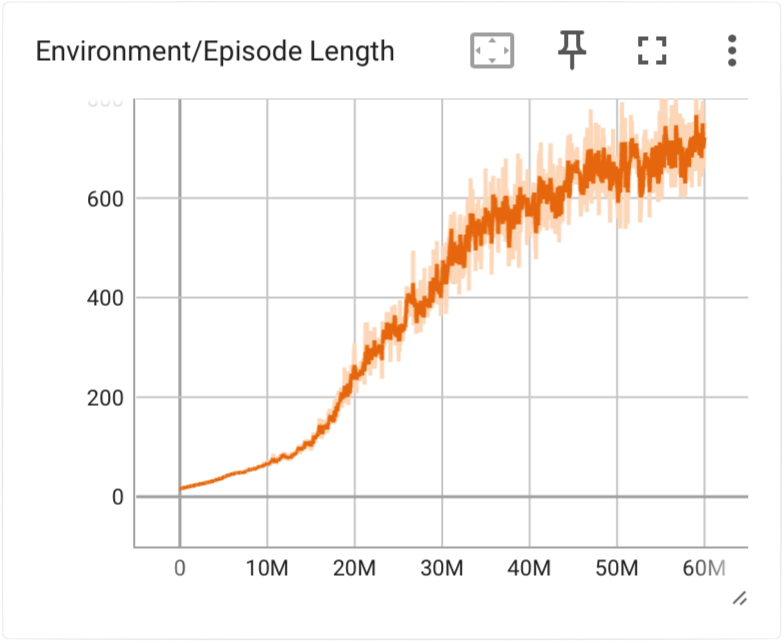
\includegraphics[width=\textwidth]{img/106_episode_length}
      \caption{Episodenlänge}
      \label{fig:106_episode_length}
    \end{subfigure}
    \begin{subfigure}{.49\textwidth}
      \centering  
      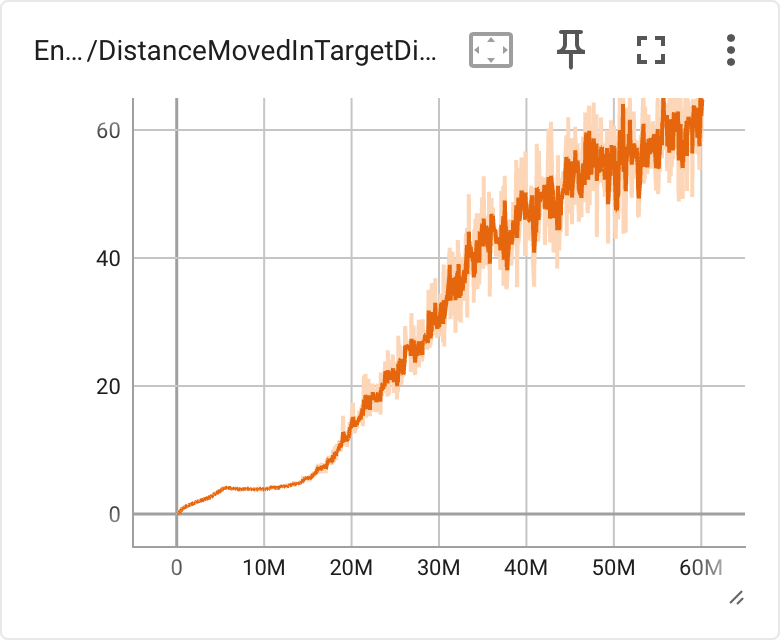
\includegraphics[width=\textwidth]{img/106_move_target_dir}
      \caption{Zurückgelegte Stecke in Zielrichtung}
      \label{fig:106_move_target_dir}
    \end{subfigure}
    \begin{subfigure}{.49\textwidth}
      \centering  
      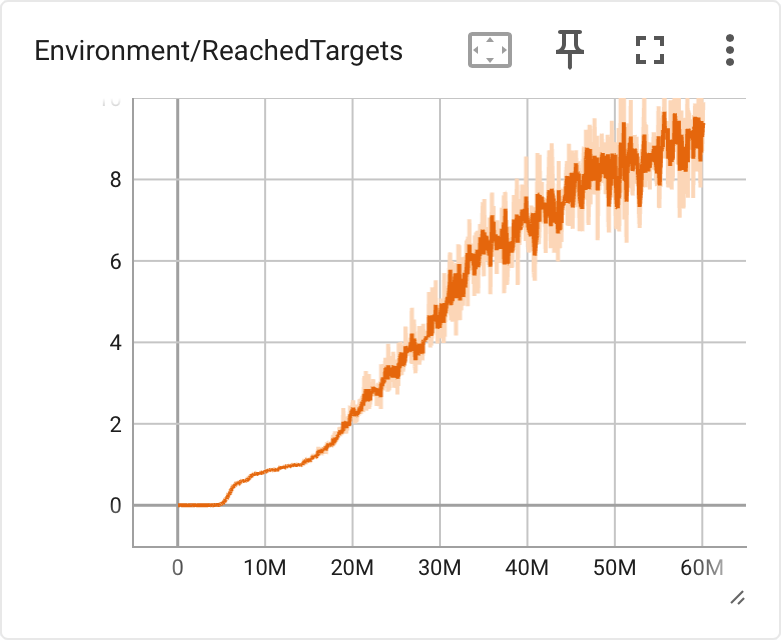
\includegraphics[width=\textwidth]{img/106_reach_target}
      \caption{Erreichte Anzahl an Zielen}
      \label{fig:106_reach_target}
    \end{subfigure}
    \begin{subfigure}{.49\textwidth}
      \centering  
      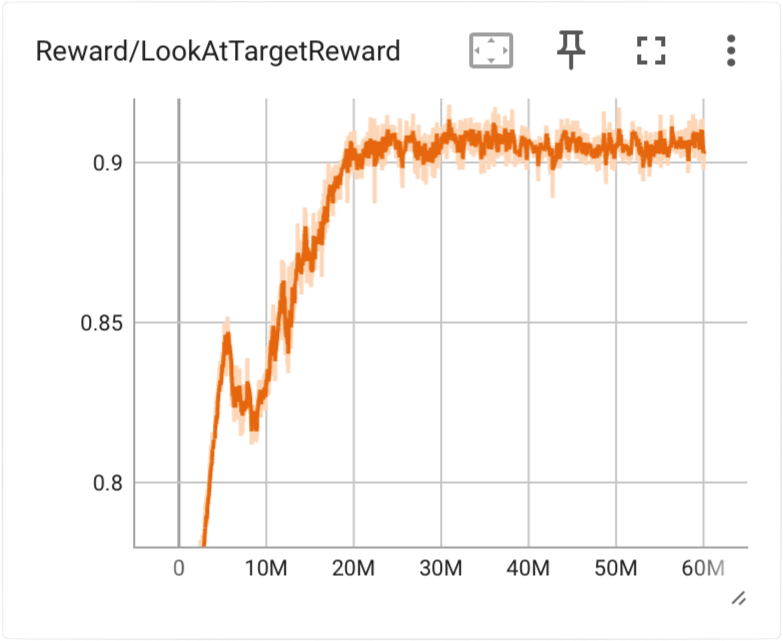
\includegraphics[width=\textwidth]{img/106_look_reward}
      \caption{Blickbelohnung}
      \label{fig:106_look_reward}
    \end{subfigure}
    \begin{subfigure}{.49\textwidth}
      \centering  
      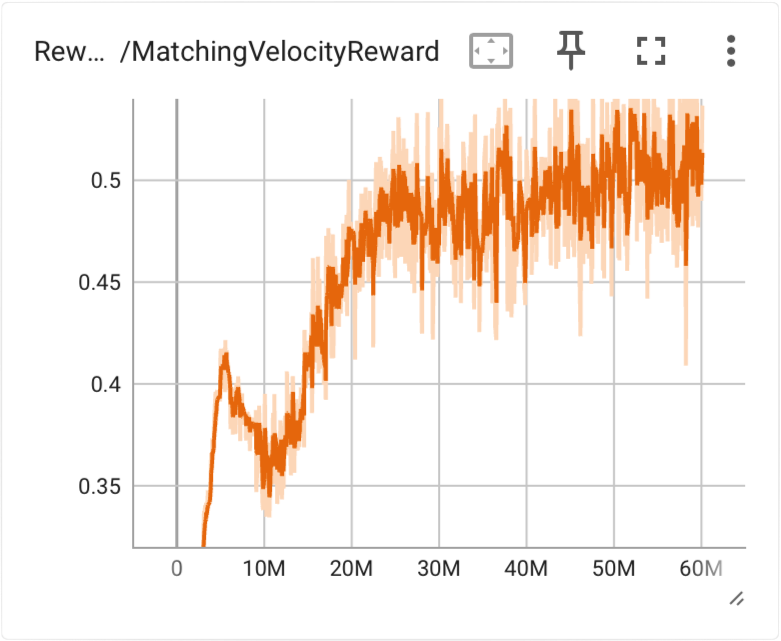
\includegraphics[width=\textwidth]{img/106_vel_reward}
      \caption{Geschwindigkeitsbelohnung}
      \label{fig:106_vel_reward}
    \end{subfigure}
 \caption{Training Mixamo Charakter}
  \label{fig:training_mixamo_charakter}
\end{figure}

\begin{figure}[H]
  \centering
  \begin{tabular}{cccc}
    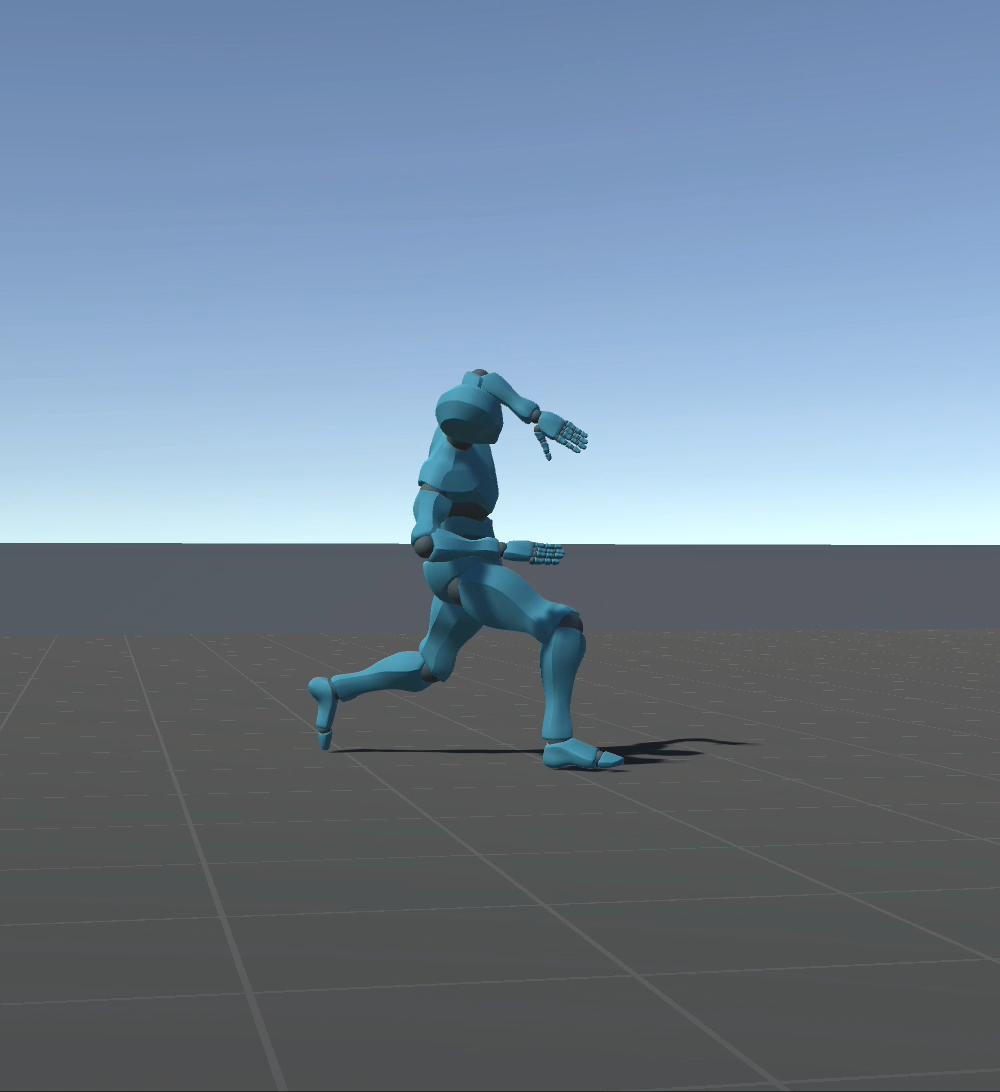
\includegraphics[width=0.2\textwidth]{img/charakter_mixamo_galoppieren1} & 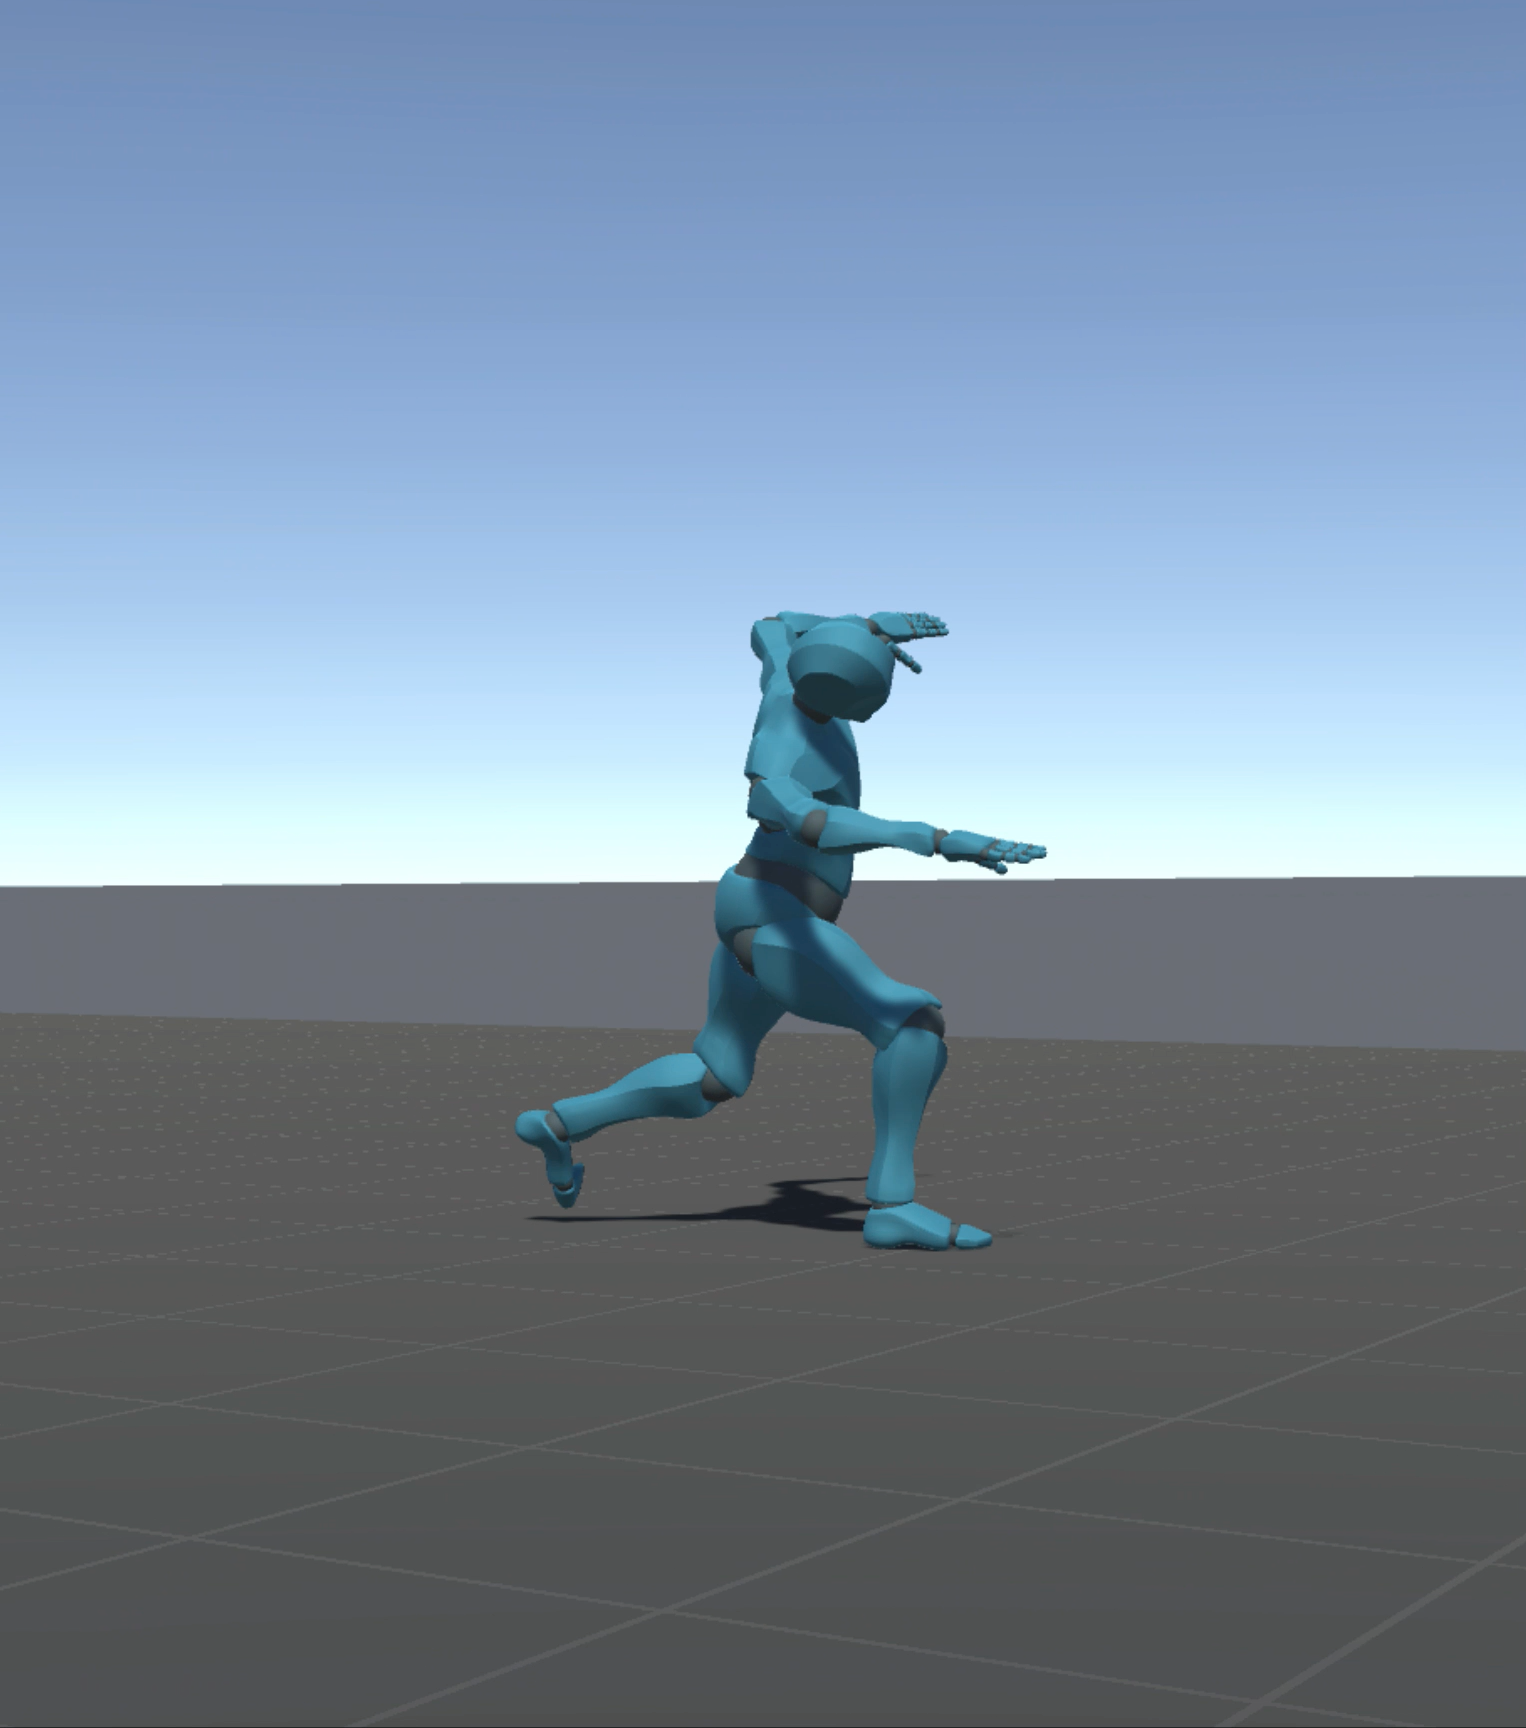
\includegraphics[width=0.2\textwidth]{img/charakter_mixamo_galoppieren2} & 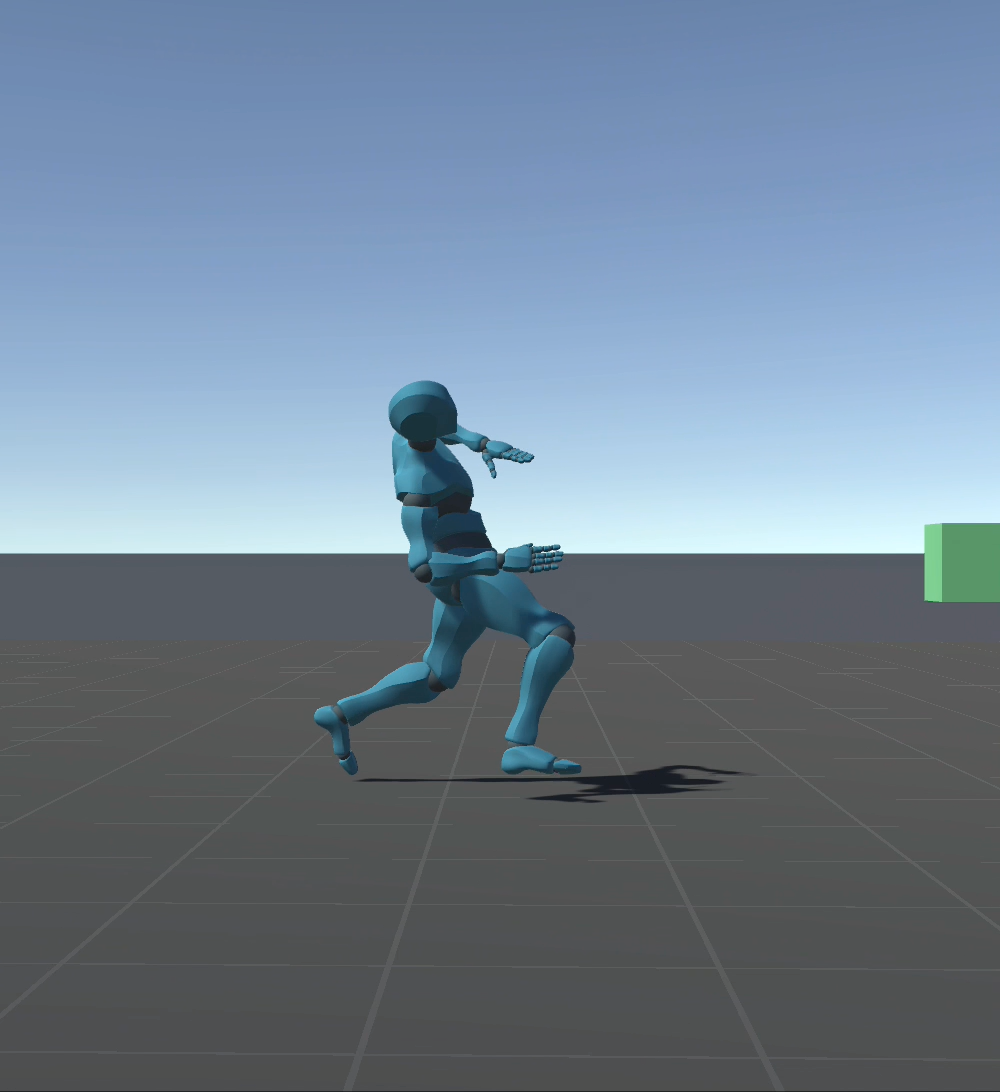
\includegraphics[width=0.2\textwidth]{img/charakter_mixamo_galoppieren3} & 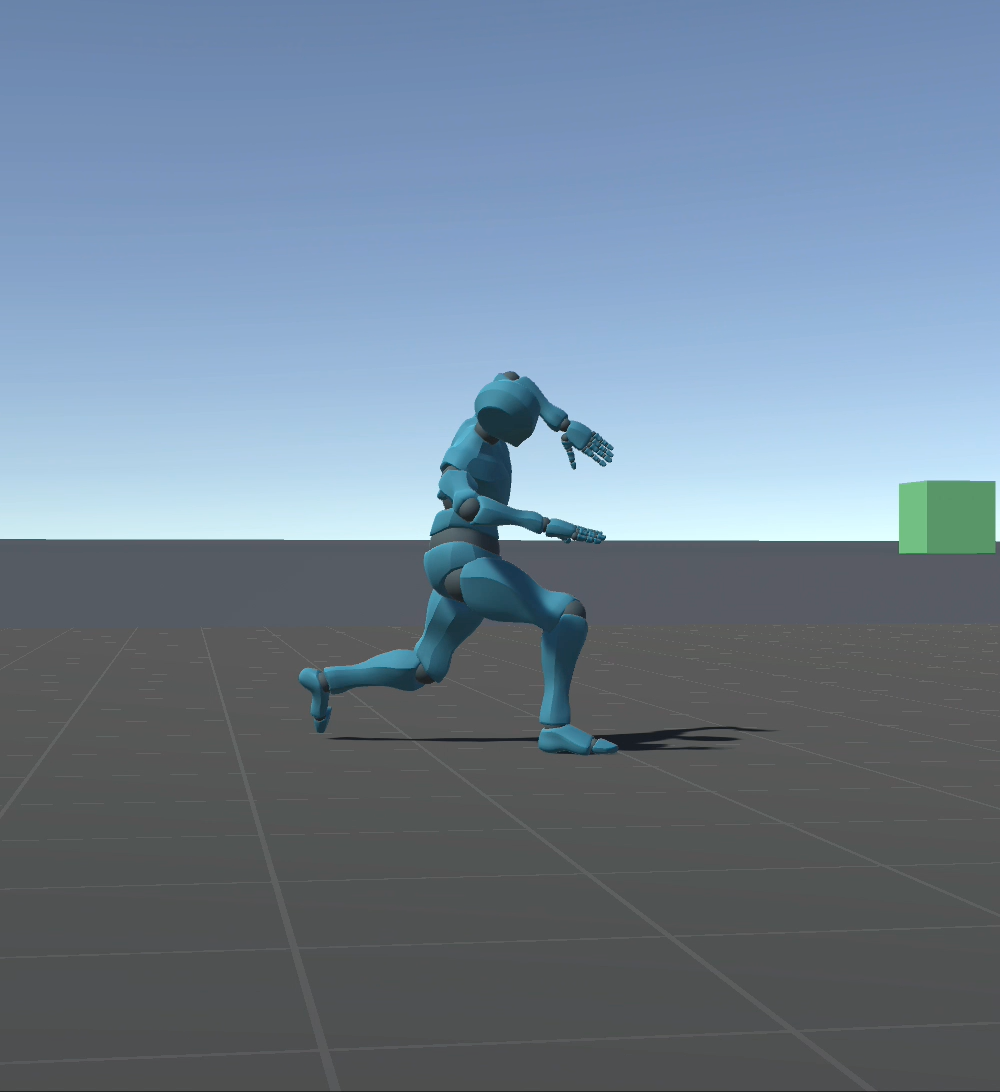
\includegraphics[width=0.2\textwidth]{img/charakter_mixamo_galoppieren4} \\
  \end{tabular}
  \caption{Mixamo Versuch 10 Gangbild}
  \label{fig:mixamo_versuch10_gangbild}
\end{figure}